 \documentclass[10pt,a4paper]{article}
\usepackage[T1]{fontenc}
\usepackage[utf8]{inputenc}
\usepackage[brazil]{babel}
\usepackage{indentfirst}
\usepackage{graphicx}
\usepackage{caption}
\usepackage[section]{placeins}
\usepackage{listings}

\begin{document}

	\title{INF01124 - Classificação e Pesquisa de Dados - Exercício 3}
	\date{}
	\author{Felipe de Almeida Graeff\\00261606}
	\maketitle

	\section{Hybrid Sort}

		A implementação do merge sort desenvolvida pode ser conferida abaixo.
		Para a utilização híbrida do algoritmo de merge com o de inserção, é avaliado 
		se o tamando da sublista que está sendo ordenada é menor ou igual ao argumento 
		$k$ fornecido. Caso positivo a sublista é ordenada utilizando-se o algoritmo 
		de insertion sort fornecido, com algumas modificações para a utilização da classe 
		\emph{vector} do C++.
		
		A escolha do valor ótimo $k$ depende de diversos fatores, como linguagem de programação 
		e implementação utilizadas. O merge sort utiliza recursão e , quando não é feito in-place, 
		memória auxiliar. O overhead gerado pelas chamadas recursivas e pelo gerenciamento da 
		memória auxiliar pode fazer com que, pricipalmente para entradas pequenas, o insertion 
		sort seja mais rápido. O valor ideal de $k$ é o menor tamanho de entrada em que, mesmo 
		com o overhead, o merge sort termina em menos tempo que o insertion sort. Como esse 
		overhead varia de acordo com a linguagem e a implementação, esse valor só pode ser obtido 
		através de experimentação.
		
		Para o cômputo dos tempos de execução mostrados no gráfico abaixo foi utilizado o valor 
		arbitrário $10$ para $k$.
		
		\lstinputlisting[caption=merge\_sort.hpp,numbers=left,firstnumber=8,language=C++, firstline=8, lastline=9]{merge_sort.hpp}
		
		\lstinputlisting[caption=merge\_sort.cpp,numbers=left,firstnumber=48,language=C++, firstline=48, lastline=71]{merge_sort.cpp}

		\captionof{figure}{Tempos de execução}
		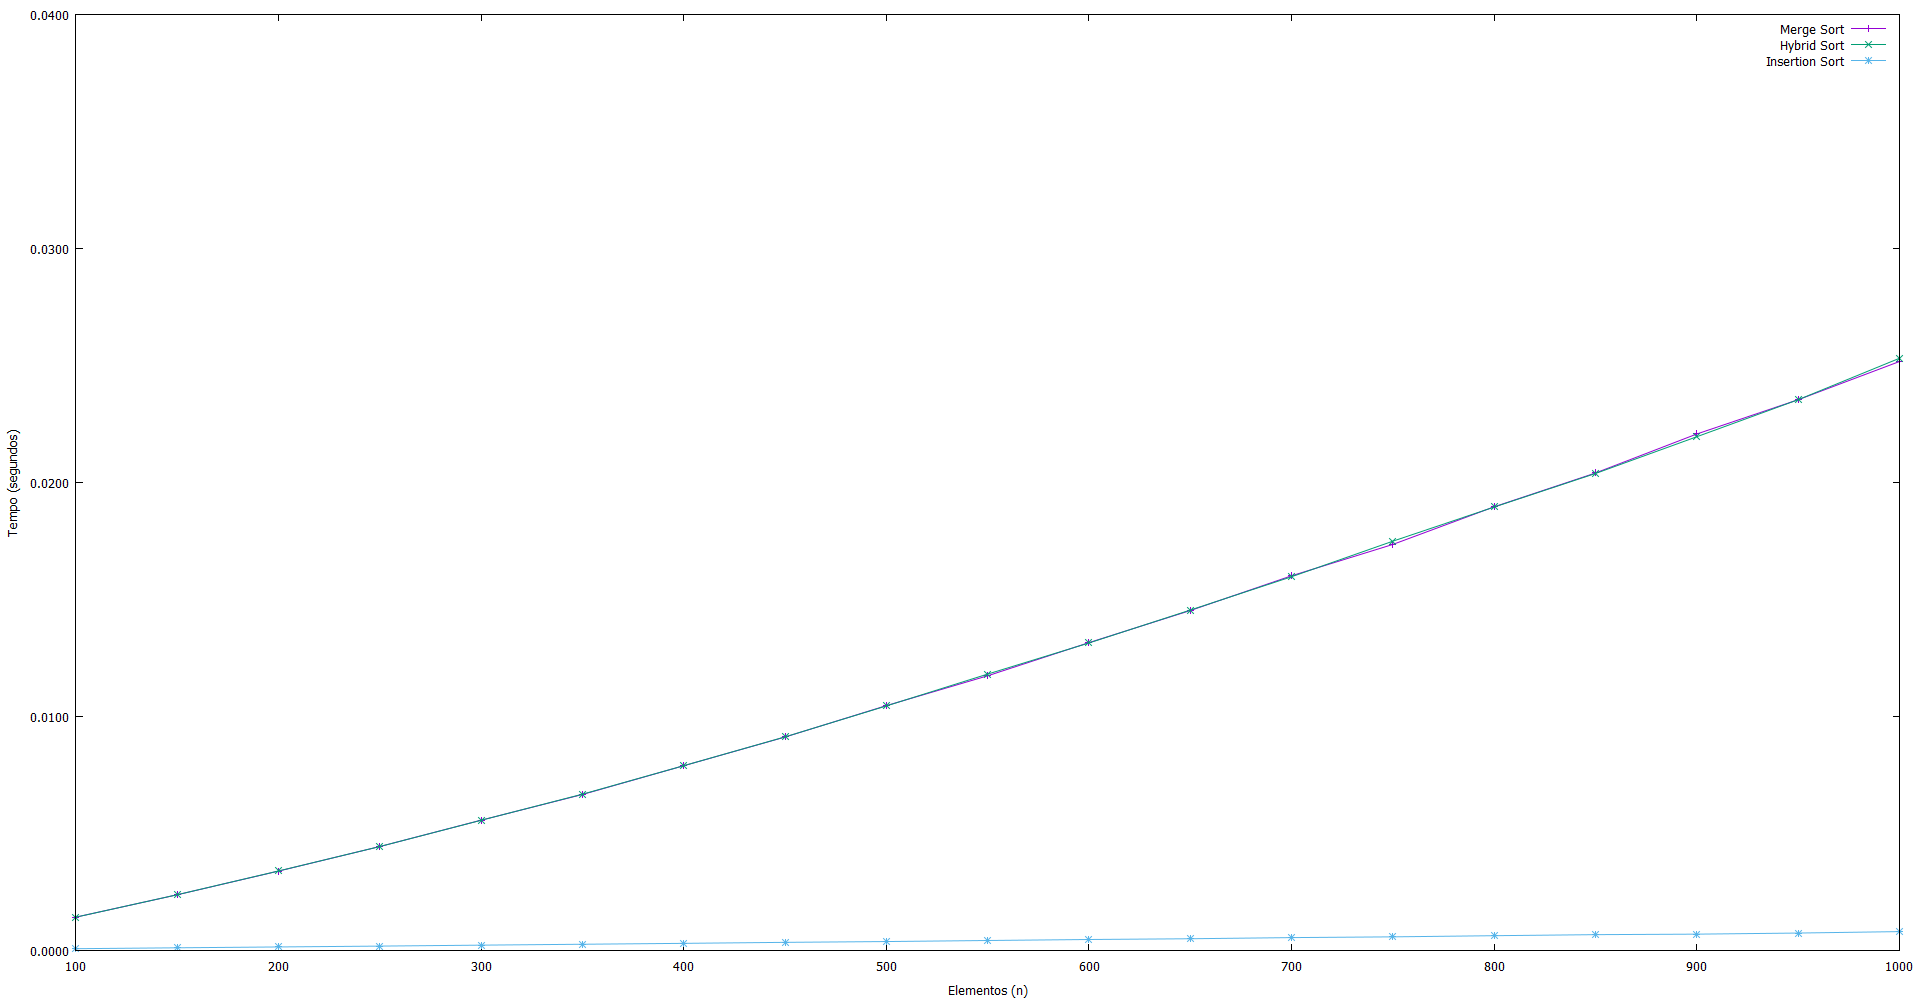
\includegraphics[width=\textwidth]{plot.png}
	
	\section{Radix Sort}
	
		A implementação do radix sort foi feita em Python e pode ser vista abaixo.
		
		O código feito pode ser dividido em 3 partes:
		
		\begin{enumerate}
	
			\item Para ordenar uma lista de inteiros positivos é executado o trecho da linha 13 
			até a linha 23. Primeiramente é calculada a quantidade de iterações necessárias 
			para a ordenação baseando-se no número de dígitos do maior elemento da lista. Após 
			isso o algoritmo de radix sort propriamente dito é executado.
			
			\item Para números de tipo \emph{float} foi utilizado o princípio de que, para números 
			em ponto flutuante de precisão simples, ou seja, de 32 bits, a precisão máxima é de 6 
			casas decimais. Portanto, nas linhas 11 e 12, todos os números da lista são multiplicados 
			por $10^6$ e transformados em inteiros. Assim obtem-se uma lista de inteiros e pode-se 
			utilizar o mesmo algoritmo do item anterior. Ao final, nas linhas 24 e 25, todos os 
			elementos da lista já ordenada são divididos por $10^6$ para que se obtenha os valores 
			originais novamente.
			
			\item Por fim, para poder ordenar também números negativos, da linha 4 à linha 9 os 
			elementos da lista inicial são divididos em uma lista de positivos e outra de negativos.
			O algoritmo dos itens anteriores foi colocado em um laço for na linha 10 que executa para 
			as duas listas. Ao final do algoritmo a lista ordenada de positivos é concatenada à lista 
			ordenada de negativos e retornada.
	
		\end{enumerate}
	
		\lstinputlisting[caption=cpdsort.py,numbers=left,firstnumber=3,language=Python, firstline=3, lastline=26]{cpdsort.py}
		
		Como o número de iterações do radix sort depende da quantidade de dígitos dos números a serem 
		ordenados, uma representação binária de um float exigiria um pior caso de 32 iterações, portanto 
		uma representação em bases maiores executaria, em teoria, mais rapidamente.
		
		Em geral, para dados númericos, a ordem lexicográfica obtida com a ordenação MSD não é interessante, 
		então o algoritmo LSD seria preferível nesse caso.
	
\end{document}
